\section{Background}
\label{s:background}

While concurrency has been a cornerstone of performance benefits in
the multicore era, it leaves a risk of malfunction, \ie, concurrency
bug, caused by insufficient thought of concurrent events.
%
In this section, we describe two types of concurrency bug, data race
and race condition, and introduce prior approaches to spot out
concurrency bugs.

\subsection{Concurrency Bug}
\label{ss:concurrencybugs}

A concurrency bug can be classified into two categories according to
how it adversely affects a program.

\begin{figure}
  \centering
  \subfloat[Data race.\label{subfig:datarace}] {
    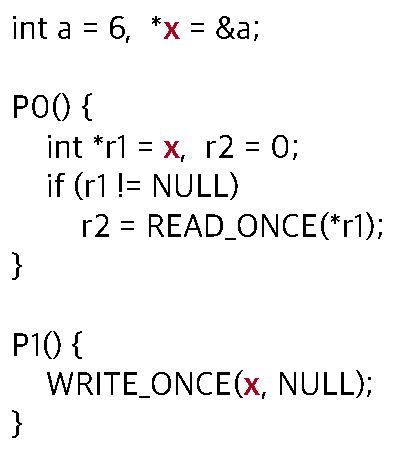
\includegraphics[width=0.45\linewidth]{fig/datarace.pdf}
  }
  \hfill
  \subfloat[Race condition.\label{subfig:racecondition}] {
    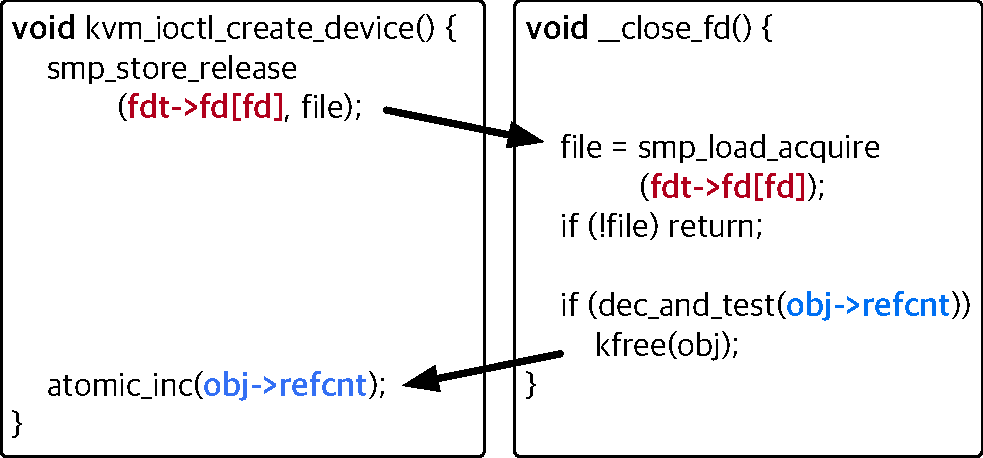
\includegraphics[width=0.45\linewidth]{fig/racecondition.pdf}
  }
  \caption{Two types of concurrency bugs.}
  \label{fig:concurrencybugs}
\end{figure}  


\PP{Data race.}
%
Although the concept of data race is well known, its formal definition
depends on a programming language~\cite{C-standard-n2310,
  java-standard} or a program in development~\cite{lkmm}. In this
paper, we employ the definition from Linux Kernel Memory Model
(LKMM)~\cite{lkmm}. According to LKMM, a data race occurs when there
are two memory accesses such that 1) they access the same location, 2)
at least one of them is a store, 3) at least one of them is not
annotated with special operations such as \texttt{WRITE_ONCE()}, or
\texttt{smp_load_acquire()}, 4) they occur on different CPUs (or in
different threads on the same CPU), and 5) they execute concurrently.
%
Informally, a data race indicates un-annotated concurrent accesses to
a shared memory location.

Data races are problematic because they may confuse a compiler.  LKMM
allows a compiler to assume that there will be no data race during the
runtime. Based on the assumption, a compiler has its rights to
arbitrarily transform plain accesses (\ie, accesses not annotated with
above operations), making the results unpredictable if there is a data
race during the runtime.
%
Therefore, LKMM defines the outcome of the program as undefined
behavior if a data race occurs.
%
Also, to prevent such undefined behaviors, LKMM requires developers to
annotate accesses if they possibly run
concurrently~\cite{data-race-fix1, data-race-fix2, data-race-fix3}.
% %
% On the other hand, data races may or may not cause a real-world issue
% such as memory corruption. Many data races fixes~\cite{data-race-fix1,
%   data-race-fix2, data-race-fix3} annotate memory accessing
% instructions with above operations, which actually does not affect the
% compiled binary.


\PP{Race condition.}
%
Race condition is another type of concurrency bug. While a race
condition broadly indicates that an outcome differs depending on the
timing of concurrent events, we restrict the definition to indicate
the correctness of the outcome differs according to the timing of
concurrent events.
%
Specifically, if developers do not take consider of all possible
interleavings, a program may execute an erroneous interleaving which
leads the program into an unintended state.
%
Immediately or after a certain amount of time, the unintended state
causes erroneous behaviors of the program such as memory corruption,
deadlock, and assertion violation.

% \dr{TODO: what more?}
% In order to fix the errorneous interelaving, developers often utilize
% synchronization primitives such as a lock, or switch the order of
% instructions in a program~\cite{learningfrommistakes}.


% https://stackoverflow.com/questions/11276259/are-data-races-and-race-condition-actually-the-same-thing-in-context-of-conc
%
\PP{Differences between data race and race condition}
%
\dr{TODO: rewrite to enphasize that finding race condition is
  important and combine this into the race condition paragraph}
%
Although both race condition and data race are a bug caused by
concurrenct events, there are a few differences.
%
First, a data race is regards to a single pair of conflicting accesses
while a race condition is about an interleaving.
%
Therefore, methods to detect them are also different.  While data race
detectors~\cite{tsan, krace, prorace, crsampler, txrace} monitor
whether two conflicting plain accesses are executed concurrently, race
conditions can be observed only through an erroneous behavior caused
by a specific interleaving.
%
Second, whereas a data race occurs if such conflicting accesses exists
no matter it causes an erroneous behavior or not, a race condition is
told by an abnormal outcome of a program.
%
% In the security perspective, a data race requires further
% investigation to determine whether it is harmful or
% not~\cite{portend, replayanalysis}, the effect of a race condition
% is exmained by erroneous behaviors such as general protection fault,
% assertion violations, sanitizers~\cite{asan, kasan} and
% lockdep~\cite{lockdep} reports.
%
% \begin{figure}
%   \centering
%   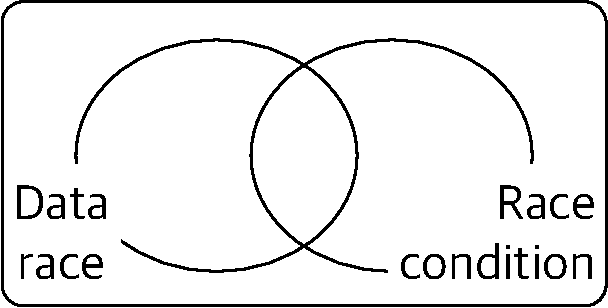
\includegraphics[width=0.45\linewidth]{fig/venndiagram.pdf}
%   \caption{Relation between data race and race condition. This paper
%     focuses on the striped region. \dr{I don't think we need this.}}
%   \label{fig:venndiagram}
% \end{figure}  
%
Lastly, they are not a subset or a superset of one another. Although
there are race conditions that occur with data races, neither one is
the sufficient nor necessary condition for the other. Therefore, we
would argue that finding data races and finding race condditions are
complementary with each other.


\PP{Scope of this paper}
%
This paper focuses on finding race conditions instead of data races.

\dr{TODO: why? want to say finding race condition is more important,
  and existing approaches to find data races are limited}

\dr{TODO: need to say the importance of observing erroneous outcomes}


\subsection{Concurrency Fuzzing}
\label{ss:concurrencyfuzzing}


% During fuzzing, a fuzzer determines that interleavings of given
% concurrent jobs are tested enough if a concurrency coverage is
% saturated while a customized scheduler is introduced to tailor the
% non-deterministic behavior.


In spite of enormous efforts, finding concurrency bugs is still a
daunting task.
%
It is mainly due to two challenges such that 1) concurrency bugs are
inherently caused non-deterministically, and 2) the number of possible
interleavings grows exponentially to the number of memory access
operations.

Recently, several studies~\cite{razzer, krace, snowboard, muzz} have
been proposed to improve fuzzing techniques specifically in exposing
concurrency bugs.
%
These studies generally adopt two strategies, namely customized
scheduler to tail the non-determinism, and coverage metric in the
concurrency dimension to capture interesting interleavings among all
possible interleavings.

\PP{Coverage-guided fuzzing}
%
Throughout decades, a fuzzing has shown its ability to find bugs in
various software layers including the userprogram space~\cite{qsym,
  driller, symsan, crfuzz, r2z2, cafl, fuzzorigin} and the kernel
space~\cite{fuzzusb, syzkaller, hfl, cabfuzz, razzer, krace, janus,
  hydra, healer}.
%
A primary task of fuzzing is to synthesize and mutate various inputs
of a target program.
%
When running the inputs, a fuzzer monitors a program's behavior, and
observes malfunctions with a help of various developer
tools~\cite{asan, kasan, meds}.

A coverage-guided fuzzer adopts a coverage metric to abstract
program's interesting behaviors.
%
During fuzzing, a fuzzer accumulates all experienced coverage as the
abstraction of tested behaviors of a program.
%
When a new input is given, a fuzzer compares coverage of the input
with the accumulated coverage to determine whether the input exposes a
new interesting behavior. If it does, a fuzzer keeps and mutates the
input to generate another input that potentially exhibits unknown
coverage.

% \dr{TODO: Do we need to tell about coverage-directed fuzzers?}

\PP{Customized scheduler.}
%
Instead of relying on the uncontrollable kernel scheduler, concurrency
fuzzing generally consists of a customized scheduler to increase the
probability of bugs being exposed.
%
Depending on how a customized scheduler schedules instructions, it is
largely categorized into randomized scheduler and scheduling
hint-directed scheduler (shortly, hint-directed scheduler).

A randomized scheduler~\cite{ski, pctalgorithm, krace, sparsernr} is
designed to randomly schedule intstructions in a disciplined
manner. It tries to keep only one thread to execute while the thread
runs until a certain number of instructions are executed or a certain
amount of time has elapsed.
%
A fuzzer and the scheduler share a small number of parameters used for
the scheduler to pseudo-randomly determine the number of instructions
or the amount of time to execute.
%
In this way, interleavings are diversified across fuzzing runs while a
fuzzer can tailor the non-determinism caused by scheduling.

On the other side, a hint-directed scheduler~\cite{razzer, snowboard}
enfoces a specific requirement of interleaving called a scheduling
hint.
%
A scheduling hint is generally in the form of an interleaving pattern
that possibly causes a concurrency bug. For example, a scheduling hint
may consists of execution order indicating a single-variable order
violation; \textit{``thread A executes a store operation writing into
  $X$ before thread B executes a load operation reading from $X$''}.
%
During fuzzing, a fuzzer keeps generating different scheduling hints,
and enforces an interleaving that contains a scheduling hint to
observe the interleaving causes an erroneous behavior.


\PP{Coverage in the concurrency dimension.}
%
To the best of our knowledge, Krace~\cite{krace} is the first work
that asserts the necessity of a coverage metric in the concurrency
dimension.
%
While many coverage metrics are proposed with their own pros and
cons~\cite{wang2019sensitive}, they only track the sequential aspect
of a program (\eg, branch coverage tracks whether a branch is taken or
not) without paying attention to communication between threads.
%
Krace states that even after sequential coverage is saturated, there
could be more interesting behaviors caused by thread interleavings,
and that if there are unexplored thread interleavings in an input, a
fuzzer should keep paying attention to the input.

To capture unique behaviors in the concurrency dimension, Krace
proposes a coverage metric called alias coverage.
%
Alias coverage tracks inter-thread data flow between a pair of
instructions. In other words, alias coverage tracks
\texttt{$I_S \rightarrow I_L$} if a load instruction \texttt{$I_L$}
reads a value written by a store instruction \texttt{$I_S$} and they
are executed in different threads.
%
% For example, if a fuzzer wants to test an interleaving that , it can
% instruct a scheduler to enfore such requirement on the two
% instructions.
%
\dr{TODO: MUZZ, and others?}
%
Although Razzer~\cite{razzer} and Snowboard~\cite{snowboard} adopt a
hint-directed scheduler, they do not make use of a concurrency
coverage metric. Therefore they do not distinguish whether two inputs
exhibit different behaviors. Instead, they concentrate on less
frequent inter-thread data flow based on an idea that those
inter-thread data flow is less likely tested and more likely causes an
abnormal behavior.

\section{Motivation}
\label{ss:motivation}

% - Coverage-guide fuzzing is important
% - How to define coverage in concurrency dimension is 
% challenging and important
% - Limitation of previous work: does not reflect 
% the nature of manifestation of race condition.

This work is motivated by an observation that prior approaches
focus on the execution order of a single pair of conflicting
accesses, but race conditions mostly are \textit{combined results of multiple pairs} 
of conflicting accesses.
%
Because of this gap\yj{xx}, prior approaches shows inefficiency in finding race
conditions.

In this section, we first describe when and how concurrency bugs
manifest to comprehend what interleavings should be tested to find
race conditions.
%
Afterwards, we identify why prior approaches are limited in finding
race conditions, and clarify our goals to address the limitations.


\PP{Manifestation of race conditions}
%
According to an extensive survey of concurrency
bugs~\cite{learningfrommistakes}, most race conditions manifest
depending on the execution order of multiple memory access operations.
%
Specifically, the study identifies that 92\% of race conditions manifest 
when at most four memory accesses operations are executed in a specific
order.
%
% For all other memory accesses, their execution orders and values
% written and read by them do not affect bugs's manifestation.

\begin{figure}[t]
  \centering
  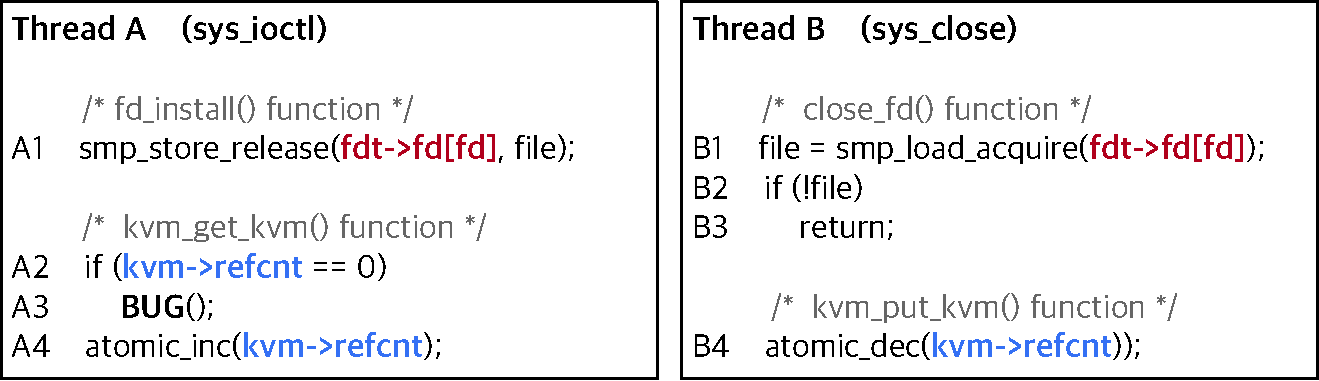
\includegraphics[width=0.95\linewidth]{fig/cve-2017-10661.pdf}
  \caption{Simplified code snippet of a NULL-dereference bug in the
    binder driver.}
  \label{fig:cve-2019-6974}
\end{figure}

\autoref{fig:cve-2019-6974} explains a case. In this example, a race
condition occurs in the binder device driver, which is an IPC
framework for Android. Specifically, a NULL-dereference bug manifests
when two system calls are executed concurrently: \texttt{mmap()} to
map the device driver into a user address space and
\texttt{ioctl(TRANSACTION)} to send an IPC message.


\yj{Are you talking about \autoref{fig:alias-coverage}?}
The race condition happens as follows. Let us suppose
\texttt{alloc->vma} and \texttt{alloc->mm} are initially
\texttt{NULL}.
%
During mapping the device driver into a user address space, thread~A
sets \texttt{alloc->vma} and \texttt{alloc->mm} to non-NULL pointers
at \texttt{A1} and \texttt{A2}.
%
However, since these two store operations are not atomically executed,
thread~B may intervene in the middle of these two instructions.
%
In that case, it is possible that \texttt{alloc->vma} is not
\texttt{NULL} when thread~B executes \texttt{B1} while
\texttt{alloc->mm} is \texttt{NULL} at \texttt{B4}.
%
As a consequnce, a NULL-dereference manifests when thread~B increments
the reference counter of \texttt{alloc->mm} at \texttt{B4}.
%
In summary, the manifestation of the race condition depends on whether
the execution order of four memory accesses meets a certain condition,
namely
$(\texttt{A1} \rightarrow \texttt{B1}) \wedge (\texttt{B4} \rightarrow
\texttt{A2})$~\footnote{In this paper, $X \rightarrow Y$ indicates that $X$
  is executed before $Y$}.

% One of the factors that makes it difficult to find concurrency bugs is
% that, they may be detected only when a program shows an abnormal
% behavior.
% %
% \autoref{subfig:racecondition} is the example of such concurrency bug.
% %
% In this example, the timing of accesses are not correctly
% contemplated. When instructions are executed in the order of
% \dr{TODO:}..., the program runs differently than the developer
% intention, causing a use-after-free bug.
% %
% However there are no plain accesses (\ie, all accesses are annotated),
% and therefore, there is no data race.
% %
% By the definition, data race detectors~\cite{tsan, kcsan, krace,
%   prorace, txrace, crsampler} are not applicable to detect this kind
% of race conditions.


% In worse cases, race conditions hardly manifest with the kernel
% scheduler. In detail, a race condition may manifest only when one
% thread stalls for a long time while another thread executes numerous
% instructions.
% %
% One could argue that those concurrency bugs are not a threat because
% it may take too long time, or even impossible to exploit.
% %
% However, a recent study, ExpRace~\cite{exprace}, reveals that an
% attacker can affect the kernel's scheduler using inter-processor
% interrupts (IPI), and exploit even such concurrency bugs.



\PP{Limitation of existing approaches}
%
In the perspective of fuzzing, a coverage metric is a paramount gear
to determine whether a given input is worthy of further mutation.
%
If a coverage metric does not represent whether an input has a
potential to trigger a race condition, a fuzzer may ignore inputs in
which there are unexplored interleavings, or waste the computing power
to valueless inputs.
%
In this regard, our primary question is whether existing coverage
metrics in the concurrency dimension are suitable to apprehend
interleavings potentially causing a race condition, for example,
$(\texttt{A1} \rightarrow \texttt{B1}) \wedge (\texttt{B4} \rightarrow
\texttt{A2})$ in \autoref{fig:cve-2019-6974}.



Unfortunately, we observe that none of existing approaches incorporate
a proper coverage metric for race conditions.
%
A few of existing approaches~\cite{snowboard, razzer} do not adopt a
coverage in the concurrency dimension at all. Therefore, they do not
make a decision as to whether a given input is worth further testing.
%
Other approaches~\cite{krace, muzz} adopt coverage metrics that are
not suitable for race conditions as they do not consider a combined
result of multiple pairs of conflicting accesses. As a consequence,
race conditions may not be exposed even after the coverages are
saturated.
%
% Consequently, existing approaches have difficulty in distinguishing a
% given input has a potential to cause an interesting behavior, \ie,
% a race condition.


\begin{figure}[t]
  \centering
  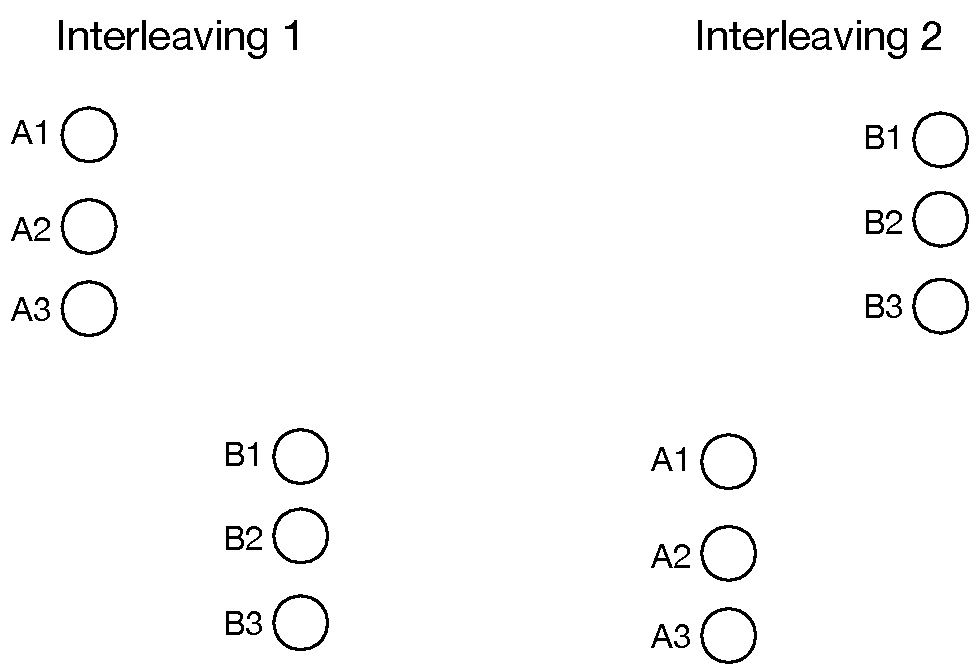
\includegraphics[width=0.98\linewidth]{fig/alias-coverage.pdf}
  \caption{Three inputs that consist of two concurrent syscalls. For
    all inputs, thread~A executes the same \texttt{mmap()} syscall
    while thread~B handles different ioctl requests. For brevity, we
    describe only conflicting instructions.}
  \label{fig:alias-coverage}
\end{figure}

\yj{This is the key paragraph to point out the limitation of previous approaches, but very vague. Make specific claims of why Kraces' alias coverage is insufficient by giving an example.}
%
In order to show why comprehending multiple pairs of conflicting
accesses is important, let us suppose we have three inputs that
consists of two concurrent syscalls as described in
\autoref{fig:alias-coverage}.
%
For all inputs, thread~A executes a \texttt{mmap()} syscall to map the
binder driver to a user address space while thread~B handles different
ioctl requests such that \texttt{ioctl(FREE_BUFFER)},
\texttt{ioctl(REPLY)}, and \texttt{ioctl(TRANSACTION)} for
\texttt{Input 1}, \texttt{Input 2}, and \texttt{Input 3} respectively.
%
It is worth noting that in \texttt{Input 1} and \texttt{Input 2},
there is only one pair of conflicting accesses; in \texttt{Input 1},
the two threads conflict on \texttt{alloc->vma}, and in \texttt{Input
  2}, the two threads conflict on \texttt{alloc->mm}.



\begin{figure}[t]
  \centering
  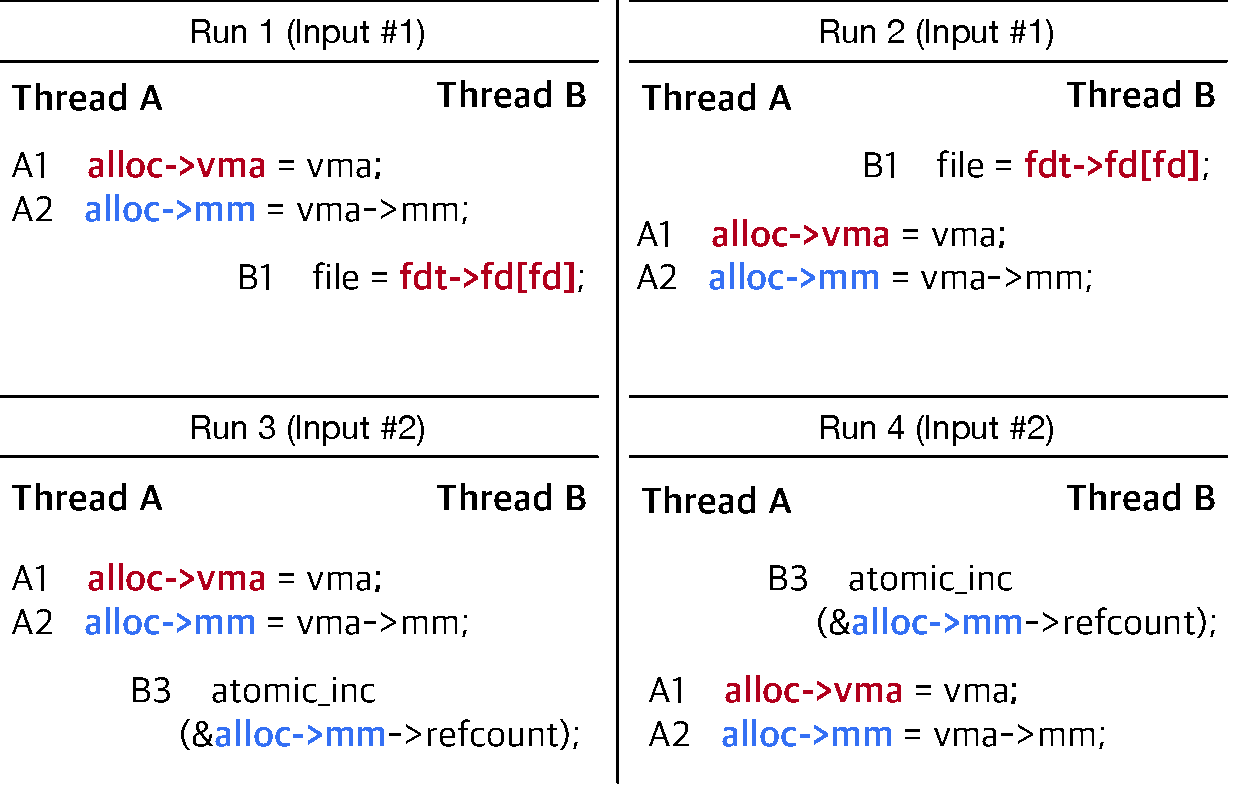
\includegraphics[width=0.9\linewidth]{fig/alias-coverage-interleaving.pdf}
  \caption{Four interleavings of \texttt{Input 1} and \texttt{Input 2}
    in \autoref{fig:alias-coverage}. After executing these four
    interleavings, all possible execution orders of a single
    conflicting accesses are exhibited.\dr{Run 1 -> Interleaving 1?}}
  \label{fig:alias-coverage-interleaving}
\end{figure}

In this example, if we adopt a coverage metric that focuses on a
single pair of conflicting accesses (\eg, alias coverage), a fuzzer
may not recognize that \texttt{Input 3} may exhibit a behavior
different than \texttt{Input 1} and \texttt{Input 2}~(\ie, a
NULL-dereference bug).
%
\autoref{fig:alias-coverage-interleaving} shows four interleavings
that exhibits all execution order of a single pair of conflicting
accesses. If a fuzzer executes \texttt{Input 1} with interleavings in
\texttt{Run 1} and \texttt{Run 2}, a fuzzer observes execution orders
such as $\texttt{A1} \rightarrow \texttt{B1}$ (in \texttt{Run 1}) and
$\texttt{B1} \rightarrow \texttt{A1}$ (in \texttt{Run 2}).
%
Similary, if a fuzzer executes \texttt{Input 2} with interleavings in
\texttt{Run 3} and \texttt{Run 4}, it observes execution orders of
$\texttt{A2} \rightarrow \texttt{B4}$ (in \texttt{Run 3}) and
$\texttt{B4} \rightarrow \texttt{A2}$ (in \texttt{Run 4}).
%
After executing these four interleavings, \texttt{Input 3} does not
reveal a new execution order of a single conflicting
accesses. Therfore, as a Krace state, a fuzzer may de-prioritize
\texttt{Input 3}, and the race condition may not be found.

In summary, in order to determine whether an input shows interesting
behaviors or not, a fuzzer needs to comprehend \textit{a combined
  result of multiple pairs of conflicting accesses} as it is the
primary reason of race conditions.


\cut{
Approaches that adopt a randomized scheduler~\cite{krace, ski, muzz}
suffer from the inherent randomness.
%
When the randomness comes to concurrency bugs, this could become a
significant drawback.
%
Although interleavings are affected by a fuzzer, a fuzzer cannot fully
control how interleaving takes place. Thus, a fuzzer may need to
indiscriminately execute the same input until its coverage is
saturated.
%
Furthermore, it is almost impossible for randomized schedulers to
expose concurrency bugs requiring an extreme interleaving such that
\dr{TODO: explain:}non-inclusive race conditions~\cite{exprace} or ones that
require a very small race window.
%
In contrast, approaches with a hint-directed scheduler is able to
explore all interelavings including even ones that hardly occur if a
proper scheduling hint is given. Therfore, they are able to find out
such race conditions.
%
However, existing approaches~\cite{razzer, snowboard} are not suitable
of diversifying interleavings. \ie, they change very small part of
interleaving across runs.
%
Even with a single input, they require a large number of execution to
test the input enough.
}

\PP{Our goal}
%
Our goal is to design a fuzzer to effectively explore the interleaving
space with a purpose of testing combinations of multiple pairs of
conflicting accesses as many as possible.
%
% Considering characteristics of concurrency bugs mentioned above, it
% will increase the probabilty of finding more concurrency bugs if we
% diversify interleavings to experience such partial orders as many as
% possible.
%
To this end, we organize subgoals as follows:
%
1) We first design a coverage metric to track combinations of pairs of
conflicting accesses,
% By this coverage metric, we do not waste the
% computing power for uninteresting inputs, and not de-prioritize inputs
% in which there are more unexplored interleavings.
%
2) based on the coverage metric, we design an interleaving mutation
mechanism that quickly saturate the coverage metric, and lastly,
%
3) we combine the coverage metric and the interleaving mutation
mechanism into Syzkaller~\cite{syzkaller} to find out race conditions
in the Linux kernel.



%
% This scheduling mechanism not only makes the investigation of such
% partial orders faster, but also does not miss concurrency bugs caused
% by an ``extreme'' interleaving (\ie, ones that hardly occur with the
% kernel scheduler).
% %
% % - observe an outcome
% %   - not to miss race conditions
% 3) While scheduling instructions, we detect concurrency bugs through
% abnormal behaviors instead of relying on data race detectors.
% %
% Although data race detectors are useful development tools, they are
% inherently limited in detecting race conditions.
% %
% We thus choose to observe the direct evidence of manifestation of
% concurrency bugs, an abnormal behavior.
% %
% Incorporating a data race detector will be discussed in
% \autoref{s:discussion}.



%%% Local Variables:
%%% mode: latex
%%% TeX-master: "p"
%%% End:
